\appendix
\chapter{Appendix}
\pagestyle{plain}
\setcounter{table}{0}
\renewcommand{\thetable}{A\arabic{table}}

\section{Parameter estimation}


\begin{figure}[h!]
\begin{center}
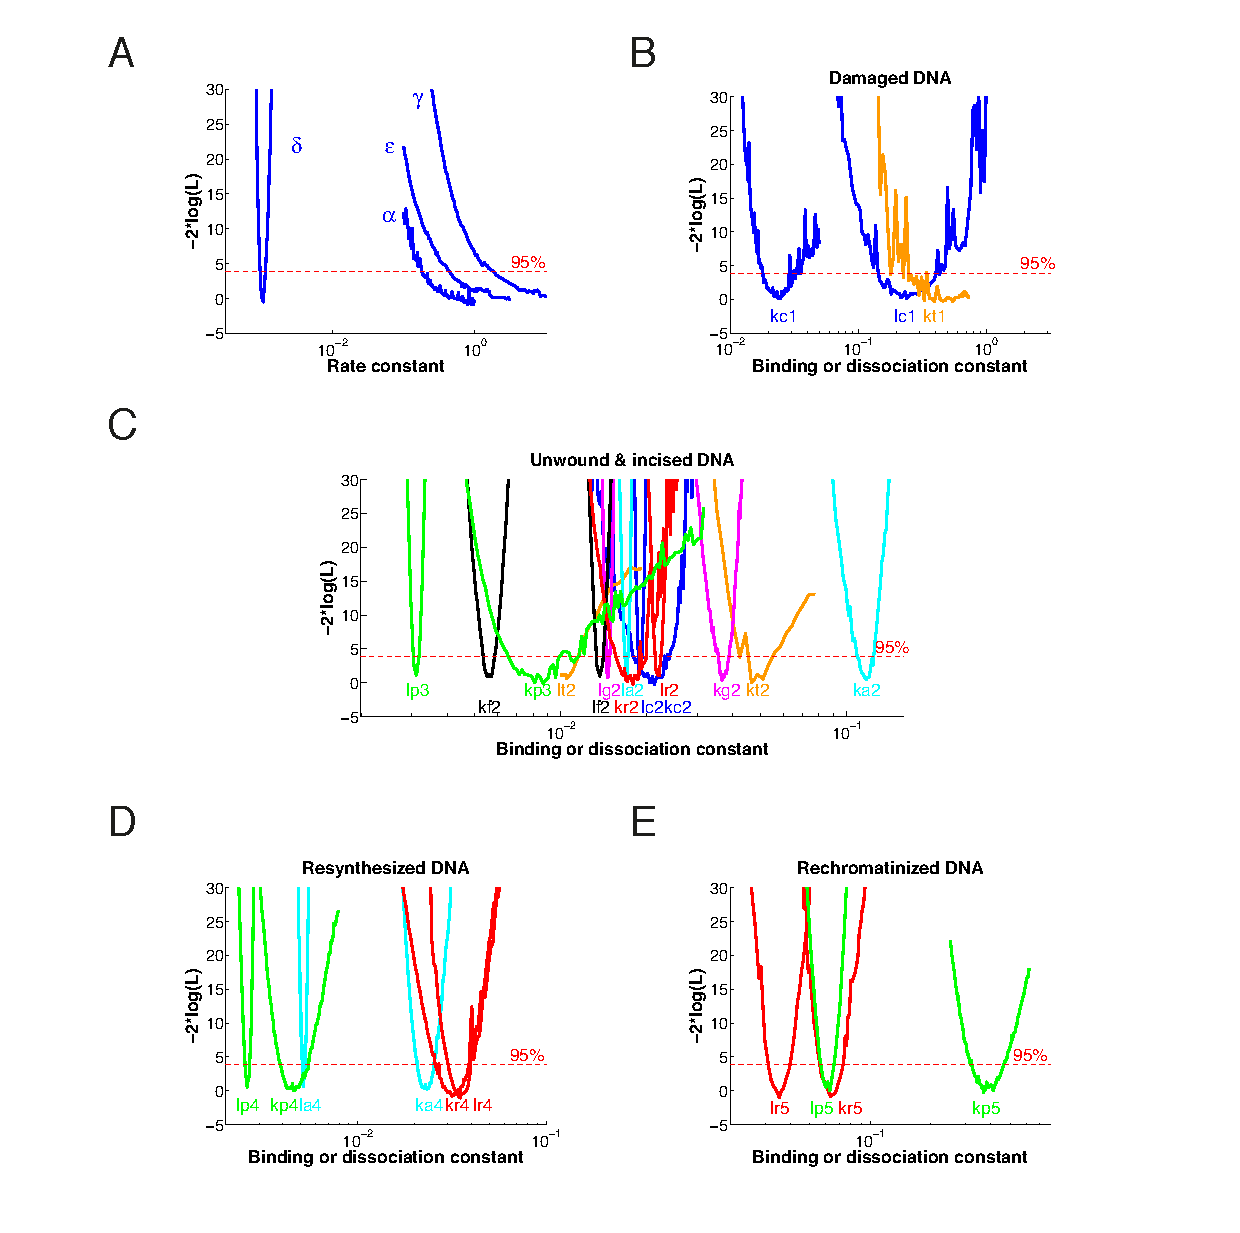
\includegraphics[width=1\textwidth]{Abbildungen/figure_A_1.pdf}
\caption{\textbf{Identifiability analysis by Profile Likelihood Estimation (PLE)} PLE and 95\% confidence interval (horizontal red line) of binding and dissociation parameters for all catalytic constants (A), damaged DNA (B), unwound and incised DNA (C), resynthesised DNA (D) and rechromatinised DNA (E). }
\label{fig:profileLikilihoods}
\end{center}
\end{figure}

\begin{table}[H]
	
	\tiny
	\begin{tabular}{lccccccc}
		
		\multicolumn{8}{l}{} \\
		\hline
		\textbf{Value}    & \textbf{ XPC} & \textbf{TFIIH} & \textbf{XPG} & \textbf{XPF} & \textbf{XPA} & \textbf{RPA} & \textbf{PCNA}  \\
		\hline
		Concentration ({\textmu}M)                                                                        &0.140    & 0.360 & 0.440& 1.110& 0.170& 1.110& 1.110     \\
		\multicolumn{8}{l}{\textbf{Damaged DNA}} \\
		$\text{k}_{\text{on}}$({\textmu}$\text{M}^{\text{-1}}\text{s}^{\text{-1}})$& 0.025               & 0.2  & NA &NA&NA&NA&NA     \\
		& (0.013;0.036)     & (0.152;0.288)  &&&&&   \\
		$\text{k}_{\text{off}}$($\text{s}^{\text{-1}})$                                             & 0.231                & 0.01 & NA &NA&NA&NA&NA     \\
		& (0.136;0.36)     &(0.009;0.012)  &&&&&   \\
		$\text{K}_{\text{d}}$({\textmu}$\text{M})$                                                  & 9.35                & 0.052  & NA &NA&NA&NA&NA     \\
		& (3.46;16.09)     &(0.044;0.072)  &&&&&   \\
		\multicolumn{8}{l}{\textbf{Unwound DNA}} \\
		$\text{k}_{\text{on}}$({\textmu}$\text{M}^{\text{-1}}\text{s}^{\text{-1}})$    & 0.022                     & 0.049                   & 0.037                 &  0.0056             & 0.116                   &0.018                    & NA    \\
		& (0.016;0.025)     & (0.04;0.06)   					&(0.036;0.039) 		 & (0.0054;0.0059)&(0.109;0.125)    &(0.016;0.02)    &     \\
		$\text{k}_{\text{off}}$($\text{s}^{\text{-1}})$                                             & 0.019                     & 0.01                   & 0.0146               & 0.0137                & 0.017                   & 0.022                   &NA     \\
		& (0.019;0.019)     & (0.009;0.012)             & (0.0140;0.0149)&(0.0134; 0.0141)&(0.0167;0.0172)     &  (0.0213;0.0224)  &   \\
		$\text{K}_{\text{d}}$({\textmu}$\text{M})$                                                  & 0.864                     & 0.204                   & 0.395                 &2.446                 &0.147                    &1.222                    &NA     \\
		& (0.635;1.006)     & (0.163;0.259)             & (0.373;0.419)		&(2.344; 2.596)&(0.138;0.158)     &  (1.048;1.36)  &   \\
		\multicolumn{8}{l}{\textbf{Incised DNA}} \\
		$\text{k}_{\text{on}}$({\textmu}$\text{M}^{\text{-1}}\text{s}^{\text{-1}})$    & 0.022                     & 0.049                   & 0.037                 &  0.0056             & 0.116                   &0.018                    & 0.008    \\
		& (0.016;0.025)     & (0.04;0.06)   					&(0.036;0.039) 		 & (0.0054;0.0059)&(0.109;0.125)    &(0.016;0.02)    	& (0.0066;0.0111)    \\
		$\text{k}_{\text{off}}$($\text{s}^{\text{-1}})$                                              & 0.019                     & 0.01                   & 0.0146               & 0.0137                & 0.017                   & 0.022                 &0.0031     \\
		& (0.019;0.019)     & (0.009;0.012)             & (0.0140;0.0149)&(0.0134; 0.0141)&(0.0167;0.0172)     &  (0.0213;0.0224)    & (0.003;0.0032)  \\
		$\text{K}_{\text{d}}$({\textmu}$\text{M})$                                                   & 0.864                     & 0.204                   & 0.395                 &2.446                 &0.147                    &1.222                   &0.388    \\
		& (0.635;1.006)     & (0.163;0.259)             & (0.373;0.419)		&(2.344; 2.596)&(0.138;0.158)     &  (1.048;1.36)  					& (0.319;0.538)   \\
		\multicolumn{8}{l}{\textbf{Resynthesized DNA}} \\
		$\text{k}_{\text{on}}$({\textmu}$\text{M}^{\text{-1}}\text{s}^{\text{-1}})$    & NA                          & NA                        & NA                      &  NA                    & 0.022                   &0.032                    &0.004    \\
		&                               &                             &                            &                          &(0.021;0.025)    &(0.025;0.037)    & (0.0038;0.005)    \\
		$\text{k}_{\text{off}}$($\text{s}^{\text{-1}})$                                             & NA                          &NA                          & NA                      & NA                     & 0.0052                  & 0.035                   &0.0026     \\
		&                               &                              &                           &                          &(0.0051;0.0053)     &  (0.031;0.042)  & (0.0025;0.0027)  \\
		$\text{K}_{\text{d}}$({\textmu}$\text{M})$                                                  & NA                          &NA                         & NA                      &NA                      &0.236                   &1.167                    &0.605     \\
		&                               &                              &                           &                          &(0.222;0.27)     &  (0.924;1.521)  & (0.531;0.747)  \\
		\multicolumn{8}{l}{\textbf{Rechromatinized DNA}} \\
		$\text{k}_{\text{on}}$({\textmu}$\text{M}^{\text{-1}}\text{s}^{\text{-1}})$    & NA                          & NA                        & NA                      &  NA                    & NA                       &0.065                    &0.396    \\
		&                               &                             &                            &                          &                            &(0.056;0.075)    & (0.359;0.457)    \\
		$\text{k}_{\text{off}}$($\text{s}^{\text{-1}})$                                             & NA                          &NA                          & NA                      & NA                     & NA                       & 0.035                   &0.061     \\
		&                               &                              &                           &                          &                            &  (0.031;0.04)  & (0.056;0.067)  \\
		$\text{K}_{\text{d}}$({\textmu}$\text{M})$                                                  & NA                          &NA                         & NA                      &NA                      &NA                         &0.538                    &0.154     \\
		&                               &                              &                           &                          &                            &  (0.438;0.645)  & (0.134;0.182)  \\
		\hline
	\end{tabular}
	\caption{\textbf{Values of binding and dissociation rate constants.} NA, not applicable. $k_{\text{on}}$, $k_{\text{off}}$ and $K_{\text{D}}$ ($k_{\text{on}}$/$k_{\text{off}}$) values are given for every repair protein and arranged in columns. Reference parameter set and 95\% confidence intervals (in parentheses) are shown. Nuclear concentration (in \textmu M) of NER factors are based on previously described data \cite{Luijsterburg2010}}
	\label{tab:parameter_bigTable}
\end{table}

\begin{table}[H]
	
\begin{center}
	\begin{tabular}{lrl}
		
		\multicolumn{3}{l}{} \\
		\hline
		\textbf{Enzymatic rate}    && \textbf{$\text{k}_{\text{cat}}$}  \\
		\hline
		&  &$\text{s}^{\text{-1}}$       \\
		Unwinding  $\alpha$                                     & 19.9& (>0.2)                 \\
		Resynthesis $\gamma$                                 & 25.5 &(>1.5)     \\
		Rechromatinization $\delta$                         & 0.001 &(0.001;0.0011)                   \\
		Reannealing  $\epsilon$                                & 5.3&(>0.9)    \\
		\hline
	\end{tabular}
	\caption{\textbf{Values of the enzymatic rate constants.}  Reference parameter set and 95\% confidence intervals (in parentheses) are shown. In case of practical non-identifiability only the lower confidence bound is given.}
	\label{tab:parameter_catalyticRates}
	\end{center}
\end{table}
\section{Control analysis}

\begin{figure}[h!]
	\begin{center}
		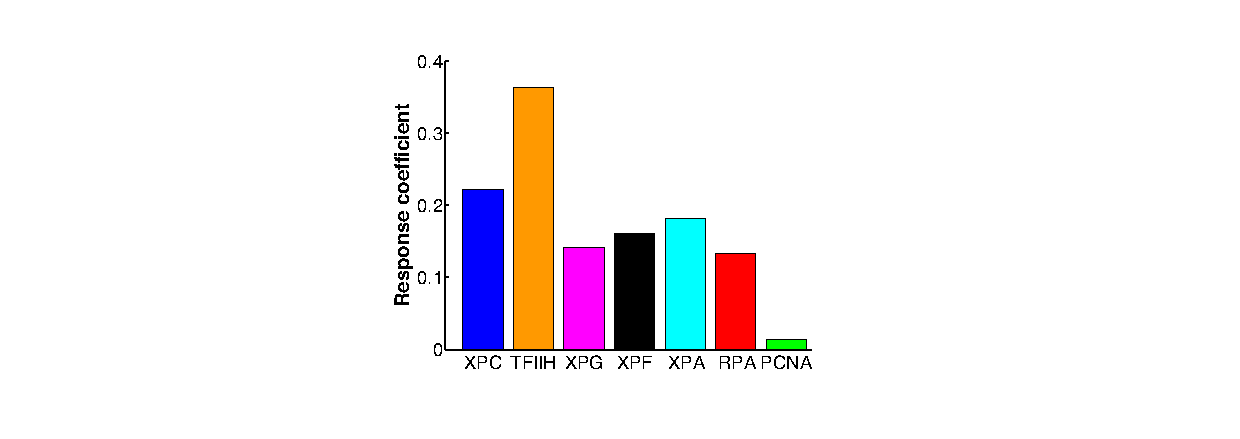
\includegraphics[width=1\textwidth]{Abbildungen/figure_A_4.pdf}
		\caption{\textbf{Uniformly distributed response coefficients for the rate of incision.} Response coefficients for the control of the incision rate by the concentrations of the repair factors. }
		\label{fig:cc_rateOfincision}
	\end{center}
\end{figure}

\newpage
\section{Cross-correlation}

\begin{figure}[h!]
	\begin{center}
		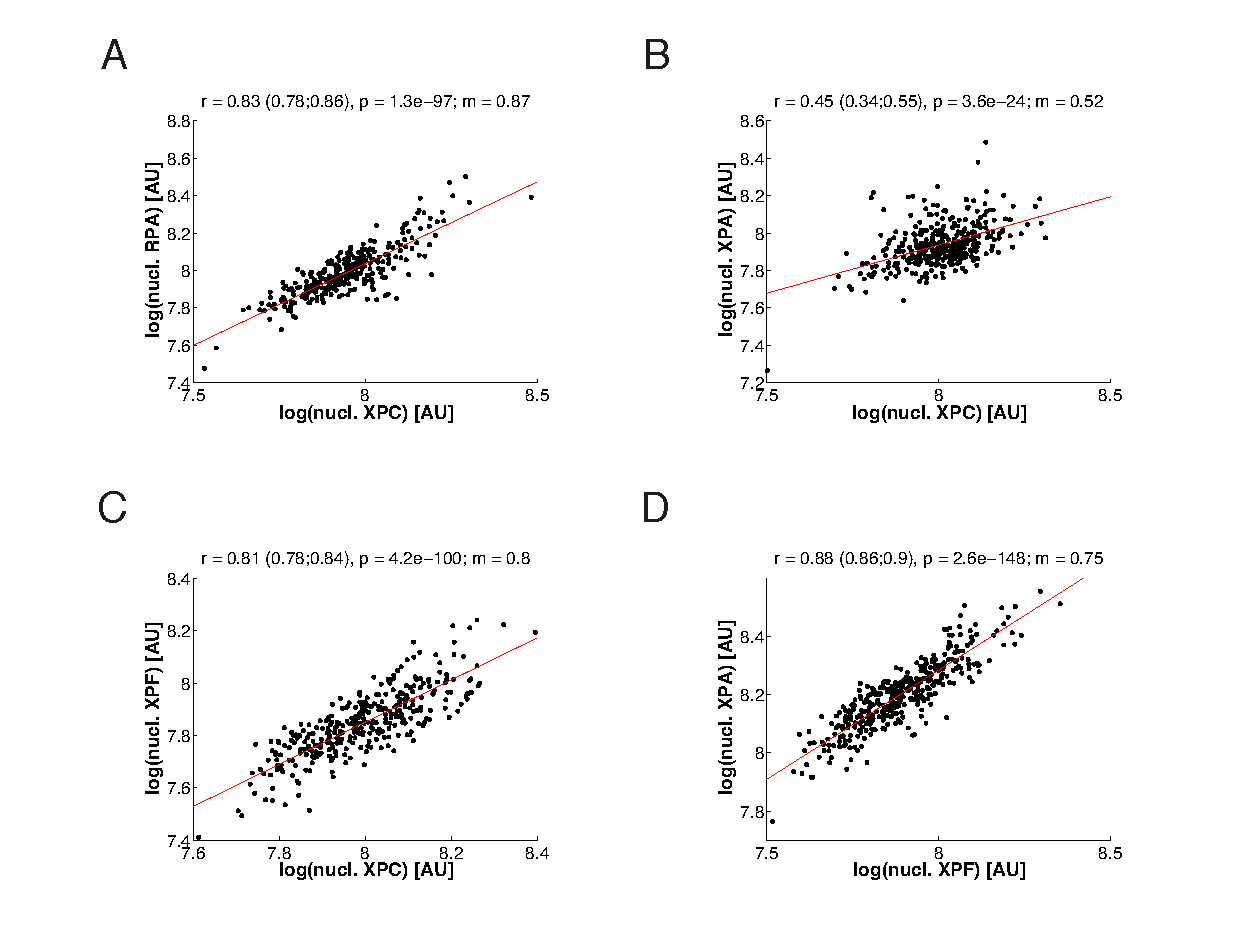
\includegraphics[width=1\textwidth]{Abbildungen/figure_A_2.pdf}
		\caption{\textbf{Nuclear expression of NER factors is correlated.} Pairwise correlations of indirectly antibody-labelled RPA against XPC (n=383, A), XPA against XPC (n=464, B), XPF against XPC (n=425, C) and XPA against XPF (n=454 , D) in locally damaged cells. Expression values represent fluorescence intensities originating from the nucleus including the damaged region. Red lines represent linear regression with correlation coefficient r, p-value and slope m. 95\% confidence bounds of all correlation coefficients r were estimated by non-parametric bootstrap and are given in brackets. }
		\label{fig:nuklearCrosscorrelation}
	\end{center}
\end{figure}
